\documentclass[12pt,a4paper]{article}
\usepackage[utf8]{inputenc}
\usepackage[T2A]{fontenc}
\usepackage[english,russian]{babel}
\usepackage{amscd}
\usepackage[dvips]{graphicx}
\usepackage{longtable,wrapfig}
\usepackage{amsfonts}
\usepackage{amsmath}
\usepackage{amssymb}
\usepackage{amsthm}
\usepackage{float}
\usepackage{mathrsfs}
\usepackage{colonequals}
\usepackage[font=small,labelfont=bf]{caption}
\usepackage[left=1in,right=1in,bottom=1in,top=1in]{geometry}
\usepackage[pdfpagelabels,hyperindex,colorlinks=true,linkcolor=blue,urlcolor=magenta,citecolor=green]{hyperref}
\usepackage{setspace}
\linespread{1.7}
\emergencystretch=1em
\usepackage{array}
\usepackage{etoolbox}
\apptocmd{\sloppy}{\hbadness 10000\relax}{}{}
\raggedbottom

%% footnote definition begins
\makeatletter
\def\keywords{\xdef\@thefnmark{}\@footnotetext}
\makeatother
%% footnote definition ends

\newtheorem{thm}{Theorem}[section]
\newtheorem{cor}[thm]{Corollary}
\newtheorem{lem}[thm]{Lemma}
\newtheorem{examp}[thm]{Example}
\newtheorem{conj}[thm]{Conjecture}
\newtheorem{defn}[thm]{Definition}

\numberwithin{equation}{section}

\title{LaTeX шаблон на русском}
\date{} %leave it blank, looks better
\author{Петро Колосов}

\hypersetup{
    pdftitle={LaTeX шаблон на русском},
    pdfsubject={
        Your Subject List
    },
    pdfauthor={Петро Колосов},
    pdfkeywords={
        Your Keywords list
    }
}

\begin{document}
    \maketitle

    \begin{abstract}
        Lorem ipsum – псевдо-латинский текст, который используется для веб дизайна, типографии, оборудования,
и распечатки вместо английского текста для того, чтобы сделать ударение не на содержание,
а на элементы дизайна.
    \end{abstract}

    \keywords{2010 \emph{Mathematics Subject Classification.} Primary ..; Secondary \dots}
    \keywords{\emph{Key words and phrases.} Ключевое слово 1, Ключевое слово 2 \dots}
    \keywords{\emph{Website.} \href{https://kolosovpetro.github.io/}{\texttt{https://kolosovpetro.github.io}}}


    \section{Введение} \label{sec:introduction}
    Текст статьи.
Пример цитирования~\cite{колмогоров1950основные, колмогоров1983комбинаторные, GithubSource_2022, Sloane_theencyclopedia}.
Lorem ipsum – псевдо-латинский текст, который используется для веб дизайна, типографии, оборудования,
и распечатки вместо английского текста для того, чтобы сделать ударение не на содержание,
а на элементы дизайна.
Такой текст также называется как заполнитель.
Это очень удобный инструмент для моделей (макетов).
Он помогает выделить визуальные элементы в документе или презентации, например текст, шрифт или разметка.
Lorem ipsum по большей части является элементом латинского текста классического автора и философа Цицерона.
Слова и буквы были заменены добавлением или сокращением элементов, поэтому будет совсем неразумно пытаться передать содержание;
это не гениально, не правильно, используется даже не понятный латинский.
Хотя Lorem ipsum напоминает классический латинский, вы не найдете никакого смысла в сказанном.
Поскольку текст Цицерона не содержит буквы K, W, или Z, что чуждо для латинского, эти буквы, а также многие другие
часто вставлены в случайном порядке, чтобы скопировать тексты различных Европейских языков, поскольку диграфы
не встречаются в оригинальных текстах.

В профессиональной сфере часто случается так, что личные или корпоративные клиенты заказывают, чтобы публикация была
сделана и представлена еще тогда, когда фактическое содержание все еще не готово.
Вспомните новостные блоги, где информация публикуется каждый час в живом порядке.
Тем не менее, читатели склонны к тому, чтобы быть отвлеченными доступным контентом, скажем, любым текстом, который
был скопирован из газеты или интернета.
Они предпочитают сконцентрироваться на тексте, пренебрегая разметкой и ее элементами.
К тому же, случайный текст подвергается риску быть неумышленно смешным или оскорбительным,
что является неприемлемым риском в корпоративной среде.
Lorem ipsum, а также ее многие варианты были использованы в работе начиная с 1960-ых, и очень даже похоже,
что еще с 16-го века.

Пример изображения
\begin{figure}[H]
    \centering
    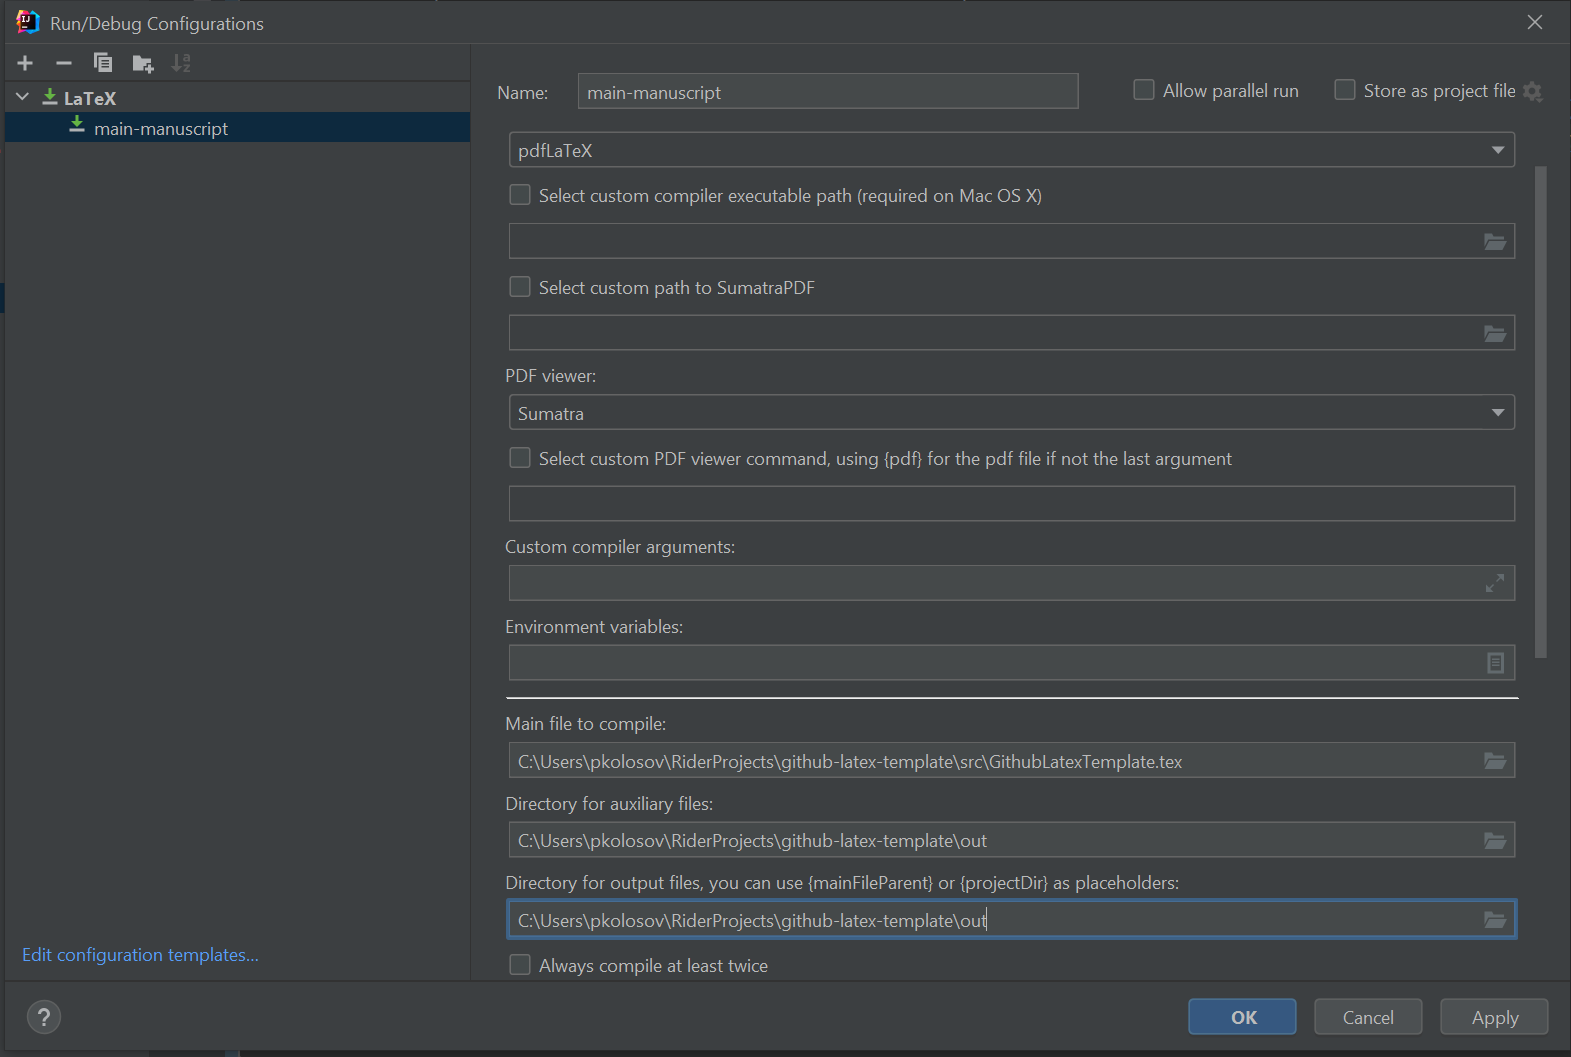
\includegraphics[width=0.8\textwidth]{../img/latex_configuration}
    ~\caption{Пример изображения.}\label{fig:figure}
\end{figure}


    \section{Заключение}\label{sec:conclusions}
    В данной статье мы рассмотрели проблему безопасного хранения и передачи токенов доступа между микросервисами.
Особое внимание было уделено возможным уязвимостям при передаче токенов доступа, таким как как Cross-Site Scripting (XSS) и Cross-Site Request Forgery (CSRF).

Для устранения данных уязвимостей необходимо хранить авторизационные токены в файлах cookie, с обязательными
настройками \texttt{HttpOnly} и \texttt{SameSite} так что значения \texttt{SameSite} должны быть \texttt{Lax} или \texttt{Strict},
таким образом файлы куки передаются либо на безопасные \texttt{HTTP} методы, либо не передаются вовсе.

Аутентификация должна быть реализована с использованием протокола OIDC~\cite{siriwardenaOpenid2020, sakimuraOpenid2014}, а Authorization code flow с помощью PKCE~\cite{bradley2015rfc}.
олее подробно основной принцип работы протокола OIDC описан в главе 2.

Аутентификация пользователя происходит по протоколу Open ID Connect~\cite{siriwardenaOpenid2020, sakimuraOpenid2014} через Authorization code flow with PKCE~\cite{bradley2015rfc}.
Подробнее принцип работы протокола Open ID Connect и Authorization code flow with PKCE изложен во главе 2.

Так же в работе был предложен механизм аутентификации/авторизации основанный на ASP.NET Web API бекенде и Angular фронтенд приложении
под единым доменом.
Таким образом исключается необходимость передачи авторизационных куки на ресурсы под другими доменами.
Передача токена доступа на микросервисы происходит по средствам Reverse Proxy YARP~\cite{microsoftYarp2021}, таким образом что
токен доступа автоматически подставляется в заголовок запроса.

Кроме того, мы предложили механизм обновления токена доступа через классы \texttt{TicketStore}~\cite{microsoftIticketstore2023} и \texttt{HostedService}~\cite{microsoftHostedservice2023}.
Таким образом, \texttt{TicketStore} проверяет каждый запрос на истечение срока действия токена доступа.
В случае истечения срока действия токена доступа он обновляется с помощью микросервиса авторизации.
Хранилище \texttt{TicketStore} также хранит пары токенов доступа и обновления внутри
\texttt{AuthenticationTicket} entity~\cite{microsoftAuthenticationTicket2023}.

Кроме этого, в работе был предложен механизм обновления токена доступа через реализацию \texttt{TicketStore}~\cite{microsoftIticketstore2023} и \texttt{HostedService}~\cite{microsoftHostedservice2023}.
Таким образом, \texttt{TicketStore} отвечает за проверку каждого запроса на истечение срока действия токена доступа.
В случае истечения срока действия токена доступа, токен доступа обновляется с помощью запроса к эндпоинту сервиса авторизации.
Также задача \texttt{TicketStore} состоит в сохранении токена доступа и токена обновления, которые являются частью \texttt{AuthenticationTicket}~\cite{microsoftAuthenticationTicket2023}.
Hosted Service необходим для фонового обновления истекающих токенов доступа, чтобы поддерживать сессии пользователей активными.

В статье мы решили проблему безопасного хранения токена доступа и передачи его между микросервисами,
а так же предложили решения выявленным уязвимостям вида Cross-Site Scripting (XSS) и Cross-Site Request Forgery (CSRF).

    \bibliographystyle{unsrt}
    \bibliography{LatexRussianTemplate}
    \noindent \textbf{Version:} \texttt{Local-0.1.0}
\end{document}